\chapter{Fundamentação Teórica}
	\label{ch:fundamentacao}
Nesta sessão serão descritos alguns dos conceitos essenciais para a compreensão do trabalho. Inicialmente sera explicado como funciona a organização Baja SAE e as provas a quais os carros são submetidos, além de um breve resumo da história da equipe Velociraptor. Também é descritos alguns detalhes técnicos de quais sensores são/devem ser aplicados no percurso do trabalho. Por ultimo algumas informações sobre os microprocessadores estudados para servir como base do \textit{SCOB} vão ser discutidas. \textbf{ATENÇÃO: VERICAR OUTRAS POSSIVEIS SEÇÕES!}

\section{Baja SAE}
A categoria Baja, organizado pela SAE (\textit{Society of Automotive Engineers}), é uma categoria de \textit{motorsport} feita para estudantes de engenharia aprofundarem seu conhecimento na área com um projeto real, no qual toda a construção do veículo deve ser realizado, bem como sua documentação e busca por patrocinadores para viabilização do projeto. Os carros a serem montados devem, por regulamento, \cite{regulamentobajasae} serem feitos de uma estrutura tubular de aço, com quatro ou mais rodas e motor padrão de 10HP. Também segundo o regulamento o carro deve suportar uma pessoa de até um metro e noventa de altura e 113,4 quilogramas de peso. Todo o sistema de suspensão, freio, transmissão e chassi é projetado e executado pela equipe participante.  

As provas realizadas pelos veículos em um torneio , segundo \cite{bajasae} são:
\begin{itemize}
	\item Segurança;
	\item Motor;
	\item Conforto;
	\item Frenagem;
	\item Suspensão;
	\item Capacidade de tração;
	\item Dirigibilidade; e
	\item Enduro.
\end{itemize}

Além destas provas a equipe também deve realizar uma apresentação com o projeto completo do veículo, contando pontos para o torneio. A equipe que obtiver a maior quantidade de pontos nas provas citadas acima ganha o torneio.

\section{Sensores}



\section{Microprocessadores}




% ------------------------------------------- PARTE DA ANDRESSA, DEIXAR PARA PEGAR ALGUM EXEMPLO DE ESCRITA
\begin{comment}
	\section{Síntese de Som}
	A síntese sonora é uma técnica de geração de som utilizando equipamentos eletrônicos ou softwares, a partir do zero. O objetivo principal não é imitar sons existentes e sim criar sons totalmente novos. Um sintetizador, um instrumento musical eletrônico como a Figura \ref{fig:sintetizador}, tem a capacidade de emitir sons de piano, flauta, violão, mas o foco é criação de novos sons com timbres diferentes. Como um sintetizador, o computador também é um ferramenta a utilizar-se na síntese sonora.

	\begin{figure}[!htb]
	\centering
		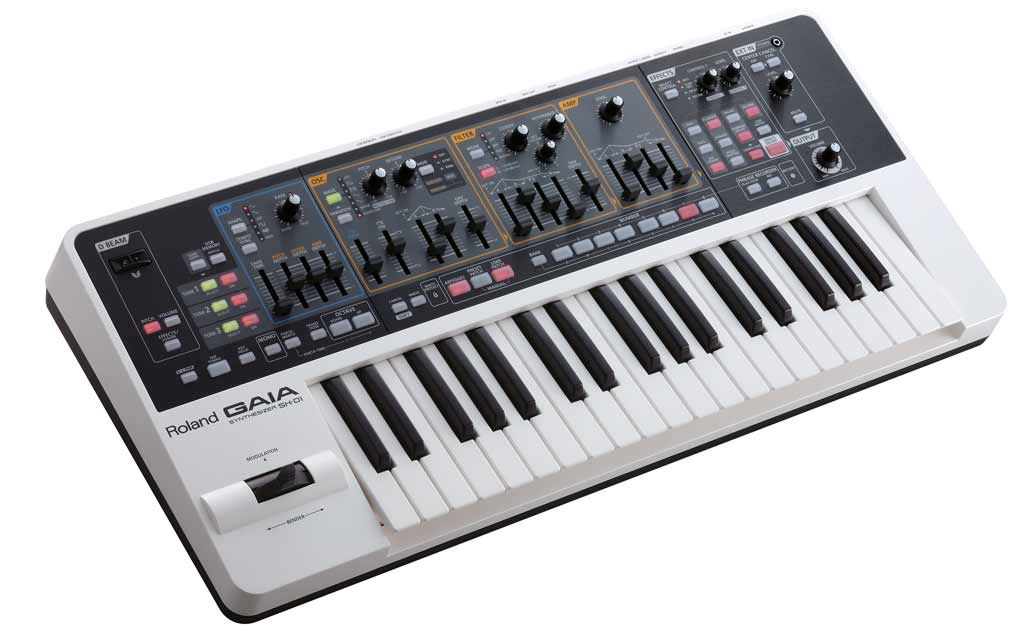
\includegraphics[height=4cm]{sintetizador}
		\caption{Exemplo de sintetizador: Roland Gaia. Fonte: Desconhecido.}
		\label{fig:sintetizador}
	\end{figure}

	Ao escolher técnicas para realizar a síntese há uma vasta gama de técnicas como síntese granular, aditiva, subtrativa entre outras.


	-----------ESCREVER MAIS


	\section{Processo Criativo}
	O processo criativo é importante para o \textit{Live Coding} pela natureza perfomática da arte, fazendo-se necessário abordar sobre composição musical e improvisação.  

	\subsection{Música}
	De acordo com \cite{lacerda1966} a música é a arte dos sons, as principais partes da música são: melodia, ritmo, harmonia.

	\begin{itemize}
		\item Melodia: o conjunto de sons dispostos em ordem sucessiva, é o tema da música, o qual capta a atenção do ouvinte;
		\item Harmonia: o conjunto de sons dispostos de forma simultânea que complementa a melodia;
		\item Ritmo: a ordem e proporção em que estão dispostos os son, definida também como a batida ou marcação do tempo.
	\end{itemize} 

	Esses elementos citados são básicos nas etapas de composição, sendo a melodia a mais importante da composição.

	\subsection{Composição musical}
	A composição musical tem como base o conhecimento do músico em relação a teoria musical e criatividade. É essencial o domínio de alguns fundamentos da teoria musical sobre a melodia, harmonia, ritmo, estilo musical, forma. A criatividade é muito influente na composição, ela está ligada com a ideias, sensibilidade do artista, ambiente onde este artista está inserido e entre outros fatores. A composição descrita aqui está ligada à criação de melodia, harmonia e definição dos instrumentos e não à criação de letra para uma música.  

	O processo da composição acontece em quatro estágios: conscientização da ideia, concepção da forma, escolha do material sonoro definindo os sons e instrumentos presentes, e estruturação estabelecendo repetições e variações sonoras. % \cite{keylist}

	Para um compositor é fundamental conseguir implementar sua criação de uma forma rápida e precisa, não por questões de produtividade, mas sim para poder reagir as suas ideias o mais próximo possível do tempo real \cite{Barbosa1999}. A tecnologia trouxe benefícios para o processo de composição musical. Os ambientes existentes para partitura e composição possibilitam que a melodia ou os arranjos criados possam ser ouvidos rapidamente com \textit{feedback}, logo após a inserção ou modificação da criação. Além de poder usar vários instrumentos diferentes na execução sem requerer a presença de um instrumentista. 	

	----Ao enfocar os processos criativos envolvidos na composição musical, argumentam que “o escasso material que tem sido escrito sobre os processos criativos (em oposição ao produto) no domínio da composição têm sido quase exclusivamente na forma de relatos pessoais [...]”. Por conseguinte, são raros os estudos que investigam os fatores que inspiram os compositores na produção de suas obras


	\subsection{Improvisação musical}	
	A improvisação musical é a arte de compor e registrar ao mesmo tempo, onde o artista expressa em tempo real as suas ideias. É necessário ter domínio do instrumento e de teoria musical, de tal maneira que consiga assimilar rapidamente a ideia e colocá-la em prática. Muitos estilos musicais são baseados na improvisação durante uma performance, Jazz , Blues e música eletrônica são exemplos que possuem essa característica marcante.
\end{comment}